\chapter{Distributions}\label{distributions}

In this chapter we'll see three ways to describe a distribution:

\begin{itemize}
\item
  A probability mass function (PMF), which represents a set of values
  and the number of times each one appears in a dataset.
\item
  A cumulative distribution function (CDF), which contains the same
  information as a PMF in a form that makes it easier to visualize, make
  comparisons, and perform some computations.
\item
  A kernel density estimate (KDE), which is like a smooth, continuous
  version of a histogram.
\end{itemize}

As examples, we'll use data from the General Social Survey (GSS) to look
at distributions of age and income, and to explore the relationship
between income and education. But we'll start with one of the most
important ideas in statistics, the distribution.

\section{Distributions}\label{distributions-1}

A distribution is a set of values and their corresponding probabilities.
For example, if you roll a six-sided die, there are six possible
outcomes -- the numbers 1 through 6 -- and they all have the same
probability, \(1/6\). We can represent this distribution of outcomes
with a table, like this:

\begin{longtable}[]{lllllll}
\toprule
Outcome & 1 & 2 & 3 & 4 & 5 & 6 \\
\midrule
\endhead
\bottomrule
\endlastfoot
Probability & 1/6 & 1/6 & 1/6 & 1/6 & 1/6 & 1/6 \\
\end{longtable}

More generally, a distribution can have any number of values, the values
can be any type, and the probabilities do not have to be equal. To
represent distributions in Python, we'll use a library called
\passthrough{\lstinline!empiricaldist!}, which stands for ``empirical
distribution'', where ``empirical'' means it is based on data rather
than a mathematical formula.

\passthrough{\lstinline!empiricaldist!} provides an object type called
\passthrough{\lstinline!Pmf!}, which stands for ``probability mass
function''. A \passthrough{\lstinline!Pmf!} object contains a set of
possible outcomes and their probabilities. For example, here's a
\passthrough{\lstinline!Pmf!} that represents the outcome of rolling a
six-sided die:

\begin{lstlisting}[language=Python,style=source]
from empiricaldist import Pmf

outcomes = [1,2,3,4,5,6]
die = Pmf(1/6, outcomes)
\end{lstlisting}

The first argument is the probability of the outcomes; the second
argument is the list of outcomes. We can display the result like this.

\begin{lstlisting}[language=Python,style=source]
die
\end{lstlisting}

\begin{tabular}{lr}
\toprule
 & probs \\
\midrule
1 & 0.166667 \\
2 & 0.166667 \\
3 & 0.166667 \\
4 & 0.166667 \\
5 & 0.166667 \\
6 & 0.166667 \\
\bottomrule
\end{tabular}

A \passthrough{\lstinline!Pmf!} object is a specialized version of a
Pandas \passthrough{\lstinline!Series!}, so it provides all of the
methods of a \passthrough{\lstinline!Series!}, plus some additional
methods we'll see soon.

\section{The General Social Survey}\label{the-general-social-survey}

We'll use \passthrough{\lstinline!Pmf!} objects to represent
distributions of values from a new dataset, the General Social Survey
(GSS). The GSS surveys a representative sample of adult residents of the
U.S. and asks questions about demographics, personal history, and
beliefs about social and political issues. It is widely used by
politicians, policy makers, and researchers.

The GSS dataset contains hundreds of columns. I've selected just a few
and save the extract in an HDF file, which is more compact than the
original fixed-width file, and faster to read. Instructions for
downloading the file are in the notebook for this chapter.

\begin{lstlisting}[language=Python,style=source]
data_file = 'gss_extract_2022.hdf'
\end{lstlisting}

We'll use the Pandas \passthrough{\lstinline!read\_hdf!} function to
read the data file and load \passthrough{\lstinline!gss!}, which is a
\passthrough{\lstinline!DataFrame!}.

\begin{lstlisting}[language=Python,style=source]
import pandas as pd

gss = pd.read_hdf(data_file, 'gss')
gss.shape
\end{lstlisting}

\begin{lstlisting}[style=output]
(72390, 9)
\end{lstlisting}

\passthrough{\lstinline!gss!} has one row for each respondent and one
column for each question in the extract. Here are the first few rows.

\begin{lstlisting}[language=Python,style=source]
gss.head()
\end{lstlisting}

\begin{tabular}{lrrrrrrrrr}
\toprule
 & year & id & age & educ & degree & sex & gunlaw & grass & realinc \\
\midrule
0 & 1972 & 1 & 23 & 16 & 3 & 2 & 1 & NaN & 18951 \\
1 & 1972 & 2 & 70 & 10 & 0 & 1 & 1 & NaN & 24366 \\
2 & 1972 & 3 & 48 & 12 & 1 & 2 & 1 & NaN & 24366 \\
3 & 1972 & 4 & 27 & 17 & 3 & 2 & 1 & NaN & 30458 \\
4 & 1972 & 5 & 61 & 12 & 1 & 2 & 1 & NaN & 50763 \\
\bottomrule
\end{tabular}

I'll explain these columns as we go along, but if you want more
information, you can read the online documentation at
\url{https://gssdataexplorer.norc.org}. In the GSS documentation, you'll
see that they use the term ``variable'' for a column that contains
answers to survey questions.

\section{Distribution of Education}\label{distribution-of-education}

To get started with this dataset, let's look at the
\passthrough{\lstinline!educ!} column, which records the number of years
of education for each respondent. We can select this column from the
\passthrough{\lstinline!DataFrame!} like this:

\begin{lstlisting}[language=Python,style=source]
educ = gss['educ']
\end{lstlisting}

To see what the distribution of the responses looks like, we can use the
\passthrough{\lstinline!hist!} method to plot a histogram.

\begin{lstlisting}[language=Python,style=source]
import matplotlib.pyplot as plt

educ.hist(grid=False)
plt.xlabel('Years of education')
plt.ylabel('Number of respondents')
plt.title('Histogram of education level');
\end{lstlisting}

\begin{center}
\includegraphics[scale=0.6666666]{08_distributions_files/08_distributions_25_0.png}
\end{center}

Based on the histogram, we can see the general shape of the distribution
and the central tendency -- it looks like the peak is near 12 years of
education. But a histogram is not the best way to visualize this
distribution because it obscures some important details.

An alternative is to use a \passthrough{\lstinline!Pmf!} object. The
function \passthrough{\lstinline!Pmf.from\_seq!} takes any kind of
sequence -- like a list, tuple, or Pandas
\passthrough{\lstinline!Series!} -- and computes the distribution of the
values.

\begin{lstlisting}[language=Python,style=source]
pmf_educ = Pmf.from_seq(educ, normalize=False)
type(pmf_educ)
\end{lstlisting}

\begin{lstlisting}[style=output]
empiricaldist.empiricaldist.Pmf
\end{lstlisting}

With the keyword argument \passthrough{\lstinline!normalize=False!}, the
result contains counts rather than probabilities. Here are the first few
values in \passthrough{\lstinline!educ!} and their counts.

\begin{lstlisting}[language=Python,style=source]
pmf_educ.head()
\end{lstlisting}

\begin{tabular}{lr}
\toprule
 & probs \\
educ &  \\
\midrule
0.000000 & 177 \\
1.000000 & 49 \\
2.000000 & 158 \\
\bottomrule
\end{tabular}

In this dataset, there are 177 respondents who report that they have no
formal education, and 49 who have only one year.

\pagebreak

Here are the last few values.

\begin{lstlisting}[language=Python,style=source]
pmf_educ.tail()
\end{lstlisting}

\begin{tabular}{lr}
\toprule
 & probs \\
educ &  \\
\midrule
18.000000 & 2945 \\
19.000000 & 1112 \\
20.000000 & 1803 \\
\bottomrule
\end{tabular}

There are 1803 respondents who report that they have 20 or more years of
formal education, which probably means they attended college and
graduate school. We can use the bracket operator to look up a value in
\passthrough{\lstinline!pmf\_educ!} and get the corresponding count.

\begin{lstlisting}[language=Python,style=source]
pmf_educ[20]
\end{lstlisting}

\begin{lstlisting}[style=output]
1803
\end{lstlisting}

Often when we make a \passthrough{\lstinline!Pmf!}, we want to know the
\emph{fraction} of respondents with each value, rather than the counts.
We can do that by setting \passthrough{\lstinline!normalize=True!}. Then
we get a \textbf{normalized} \passthrough{\lstinline!Pmf!}, which means
that the fractions add up to 1.

\begin{lstlisting}[language=Python,style=source]
pmf_educ_norm = Pmf.from_seq(educ, normalize=True)
pmf_educ_norm.head()
\end{lstlisting}

\begin{tabular}{lr}
\toprule
 & probs \\
educ &  \\
\midrule
0.000000 & 0.002454 \\
1.000000 & 0.000679357 \\
2.000000 & 0.00219058 \\
\bottomrule
\end{tabular}

Now if we use the bracket operator to look up a value, the result is a
fraction rather than a count.

\begin{lstlisting}[language=Python,style=source]
pmf_educ_norm[20]
\end{lstlisting}

\begin{lstlisting}[style=output]
0.0249975737241255
\end{lstlisting}

The result indicates that about 2.5\% of the respondents have 20 years
of education. But we can also interpret this result as a probability --
if we choose a random respondent, the probability is 2.5\% that they
have 20 years of education.

When a \passthrough{\lstinline!Pmf!} contains probabilities, we can say
that it represents a proper probability mass function, or PMF. With
apologies for confusing notation, I'll use \passthrough{\lstinline!Pmf!}
to mean a kind of Python object, and PMF to mean the concept of a
probability mass function.

\passthrough{\lstinline!Pmf!} provides a \passthrough{\lstinline!bar!}
method that plots the values and their probabilities as a bar chart.

\begin{lstlisting}[language=Python,style=source]
pmf_educ_norm.bar(label='educ')

plt.xlabel('Years of education')
plt.xticks(range(0, 21, 4))
plt.ylabel('PMF')
plt.title('Distribution of years of education')
plt.legend();
\end{lstlisting}

\begin{center}
\includegraphics[scale=0.6666666]{08_distributions_files/08_distributions_39_0.png}
\end{center}

In this figure, we can see that the most common value is 12 years, but
there are also peaks at 14 and 16, which correspond to two and four
years of college. For this data, plotting the
\passthrough{\lstinline!Pmf!} is probably a better choice than the
histogram. The \passthrough{\lstinline!Pmf!} shows all unique values, so
we can see where the peaks are.

\textbf{Exercise:} Let's look at the \passthrough{\lstinline!year!}
column in the \passthrough{\lstinline!DataFrame!}, which represents the
year each respondent was interviewed. Make an unnormalized
\passthrough{\lstinline!Pmf!} for \passthrough{\lstinline!year!} and
plot the result as a bar chart. Use the bracket operator to look up the
number of respondents interviewed in 2022.

\section{Cumulative Distribution
Functions}\label{cumulative-distribution-functions}

If we compute the cumulative sum of a PMF, the result is a cumulative
distribution function (CDF). To see what that means, and why it is
useful, let's look at a simple example. Suppose we have a sequence of
five values.

\begin{lstlisting}[language=Python,style=source]
values = 1, 2, 2, 3, 5
\end{lstlisting}

\pagebreak

Here's the \passthrough{\lstinline!Pmf!} of these values.

\begin{lstlisting}[language=Python,style=source]
pmf = Pmf.from_seq(values)
pmf
\end{lstlisting}

\begin{tabular}{lr}
\toprule
 & probs \\
\midrule
1 & 0.2 \\
2 & 0.4 \\
3 & 0.2 \\
5 & 0.2 \\
\bottomrule
\end{tabular}

If you draw a random value from \passthrough{\lstinline!values!}, the
\passthrough{\lstinline!Pmf!} tells you the chance of getting
\passthrough{\lstinline!x!}, for any value of
\passthrough{\lstinline!x!}.

\begin{itemize}
\item
  The probability of the value \passthrough{\lstinline!1!} is
  \passthrough{\lstinline!0.2!},
\item
  The probability of the value \passthrough{\lstinline!2!} is
  \passthrough{\lstinline!0.4!}, and
\item
  The probabilities for \passthrough{\lstinline!3!} and
  \passthrough{\lstinline!5!} are \passthrough{\lstinline!0.2!} each.
\end{itemize}

The \passthrough{\lstinline!Pmf!} object has a method called
\passthrough{\lstinline!make\_cdf!} that computes the cumulative sum of
the probabilities in the \passthrough{\lstinline!Pmf!} and returns a
\passthrough{\lstinline!Cdf!} object.

\begin{lstlisting}[language=Python,style=source]
cdf = pmf.make_cdf()
cdf
\end{lstlisting}

\begin{tabular}{lr}
\toprule
 & probs \\
\midrule
1 & 0.2 \\
2 & 0.6 \\
3 & 0.8 \\
5 & 1 \\
\bottomrule
\end{tabular}

If you draw a random value from \passthrough{\lstinline!values!}, the
\passthrough{\lstinline!Cdf!} tells you the chance of getting a value
\emph{less than or equal to} \passthrough{\lstinline!x!}, for any given
\passthrough{\lstinline!x!}.

\begin{itemize}
\item
  The \passthrough{\lstinline!Cdf!} of \passthrough{\lstinline!1!} is
  \passthrough{\lstinline!0.2!} because one of the five values is less
  than or equal to 1,
\item
  The \passthrough{\lstinline!Cdf!} of \passthrough{\lstinline!2!} is
  \passthrough{\lstinline!0.6!} because three of the five values are
  less than or equal to \passthrough{\lstinline!2!},
\item
  The \passthrough{\lstinline!Cdf!} of \passthrough{\lstinline!3!} is
  \passthrough{\lstinline!0.8!} because four of the five values are less
  than or equal to \passthrough{\lstinline!3!},
\item
  The \passthrough{\lstinline!Cdf!} of \passthrough{\lstinline!5!} is
  \passthrough{\lstinline!1.0!} because all of the values are less than
  or equal to \passthrough{\lstinline!5!}.
\end{itemize}

If we make a \passthrough{\lstinline!Cdf!} from a proper
\passthrough{\lstinline!Pmf!}, where the probabilities add up to 1, the
result represents a proper CDF. As with \passthrough{\lstinline!Pmf!}
and PMF, I'll use \passthrough{\lstinline!Cdf!} to refer to a Python
object and CDF to refer to the concept.

\section{CDF of Age}\label{cdf-of-age}

To see why CDFs are useful, let's consider the distribution of ages for
respondents in the General Social Survey. The column we'll use is
\passthrough{\lstinline!age!}.

According to the codebook, the range of the values is from
\passthrough{\lstinline!18!} to \passthrough{\lstinline!89!}, where
\passthrough{\lstinline!89!} means ``89 or older''. The special codes
\passthrough{\lstinline!98!} and \passthrough{\lstinline!99!} mean
``Don't know'' and ``Didn't answer''. We can use
\passthrough{\lstinline!replace!} to replace the special codes with
\passthrough{\lstinline!NaN!}.

\begin{lstlisting}[language=Python,style=source]
age = gss['age']
\end{lstlisting}

\passthrough{\lstinline!empiricaldist!} provides a
\passthrough{\lstinline!Cdf.from\_seq!} function that takes any kind of
sequence and computes the CDF of the values.

\begin{lstlisting}[language=Python,style=source]
from empiricaldist import Cdf

cdf_age = Cdf.from_seq(age)
\end{lstlisting}

The result is a \passthrough{\lstinline!Cdf!} object, which provides a
method called \passthrough{\lstinline!plot!} that plots the CDF as a
line.

\begin{lstlisting}[language=Python,style=source]
cdf_age.plot()

plt.xlabel('Age (years)')
plt.ylabel('CDF')
plt.title('Distribution of age');
\end{lstlisting}

\begin{center}
\includegraphics[scale=0.6666666]{08_distributions_files/08_distributions_56_0.png}
\end{center}

The x-axis is the ages, from 18 to 89. The y-axis is the cumulative
probabilities, from 0 to 1.

\pagebreak

The \passthrough{\lstinline!Cdf!} object can
be used as a function, so if you give it an age, it returns the
corresponding probability in a NumPy array.

\begin{lstlisting}[language=Python,style=source]
q = 51
p = cdf_age(q)
p
\end{lstlisting}

\begin{lstlisting}[style=output]
array(0.62121445)
\end{lstlisting}

\passthrough{\lstinline!q!} stands for ``quantity'', which is another
name for a value in a distribution. \passthrough{\lstinline!p!} stands
for probability, which is the result. In this example, the quantity is
age 51, and the corresponding probability is about 0.62. That means that
about 62\% of the respondents are age 51 or younger. The arrow in the
following figure shows how you could read this value from the CDF, at
least approximately.



\begin{center}
\includegraphics[scale=0.6666666]{08_distributions_files/08_distributions_61_0.png}
\end{center}

The CDF is an invertible function, which means that if you have a
probability, \passthrough{\lstinline!p!}, you can look up the
corresponding quantity, \passthrough{\lstinline!q!}. The
\passthrough{\lstinline!Cdf!} object provides a method called
\passthrough{\lstinline!inverse!} that computes the inverse of the
cumulative distribution function.

\begin{lstlisting}[language=Python,style=source]
p1 = 0.25
q1 = cdf_age.inverse(p1)
q1
\end{lstlisting}

\begin{lstlisting}[style=output]
array(32.)
\end{lstlisting}

In this example, we look up the probability 0.25 and the result is 32.
That means that 25\% of the respondents are age 32 or less. Another way
to say the same thing is ``age 32 is the 25th percentile of this
distribution''.

\pagebreak

If we look up probability 0.75, it returns 60, so 75\% of the
respondents are 60 or younger.

\begin{lstlisting}[language=Python,style=source]
p2 = 0.75
q2 = cdf_age.inverse(p2)
q2
\end{lstlisting}

\begin{lstlisting}[style=output]
array(60.)
\end{lstlisting}

In the following figure, the arrows show how you could read these values
from the CDF.



\begin{center}
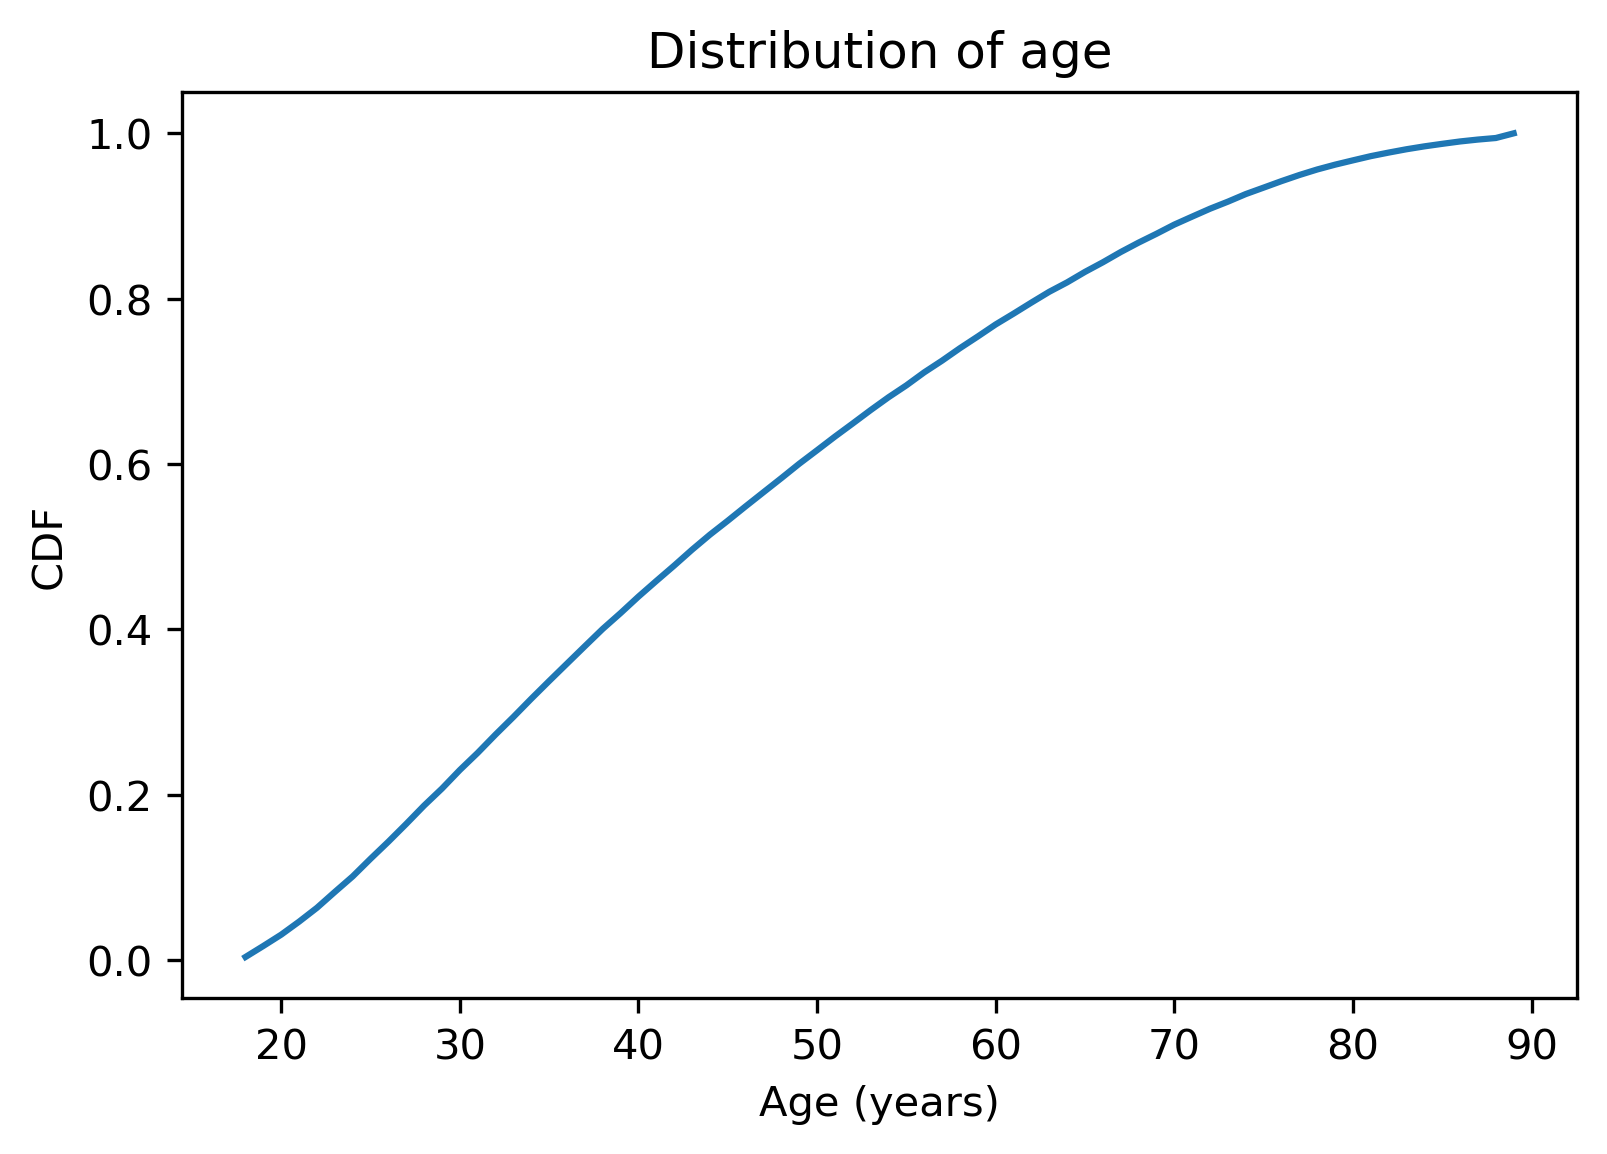
\includegraphics[scale=0.6666666]{08_distributions_files/08_distributions_67_0.png}
\end{center}

The distance from the 25th to the 75th percentile is called the
\textbf{interquartile range} or IQR. It measures the spread of the
distribution, so it is similar to standard deviation or variance.
Because it is based on percentiles, it doesn't get thrown off by
outliers as much as standard deviation does. So IQR is more
\textbf{robust} than variance, which means it works well even if there
are errors in the data or extreme values.

\textbf{Exercise:} Using \passthrough{\lstinline!cdf\_age!}, compute the
fraction of respondents in the GSS dataset who are \emph{older} than
\passthrough{\lstinline!65!}. Recall that the CDF computes the fraction
who are less than or equal to a value, so the complement is the fraction
who exceed a value.

\textbf{Exercise:} The distribution of income in almost every country is
long-tailed, which means there are a small number of people with very
high incomes. In the GSS dataset, the \passthrough{\lstinline!realinc!}
column represents total household income, converted to 1986 dollars. We
can get a sense of the shape of this distribution by plotting the CDF.
Select \passthrough{\lstinline!realinc!} from the
\passthrough{\lstinline!gss!} dataset, make a
\passthrough{\lstinline!Cdf!} called
\passthrough{\lstinline!cdf\_income!}, and plot it. Remember to label
the axes!

Because the tail of the distribution extends to the right, the mean is
greater than the median. Use the \passthrough{\lstinline!Cdf!} object to
compute the fraction of respondents whose income is at or below the
mean.

\section{Comparing Distributions}\label{comparing-distributions}

So far we've seen two ways to represent distributions, PMFs and CDFs.
Now we'll use PMFs and CDFs to compare distributions, and we'll see the
pros and cons of each. One way to compare distributions is to plot
multiple PMFs on the same axes. For example, suppose we want to compare
the distribution of age for male and female respondents. First we'll
create a Boolean \passthrough{\lstinline!Series!} that's true for male
respondents and another that's true for female respondents.

\begin{lstlisting}[language=Python,style=source]
male = (gss['sex'] == 1)
female = (gss['sex'] == 2)
\end{lstlisting}

We can use these \passthrough{\lstinline!Series!} to select ages for
male and female respondents.

\begin{lstlisting}[language=Python,style=source]
male_age = age[male]
female_age = age[female]
\end{lstlisting}

And plot a PMF for each.

\begin{lstlisting}[language=Python,style=source]
pmf_male_age = Pmf.from_seq(male_age)
pmf_male_age.plot(label='Male')

pmf_female_age = Pmf.from_seq(female_age)
pmf_female_age.plot(label='Female')

plt.xlabel('Age (years)')
plt.ylabel('PMF')
plt.title('Distribution of age by sex')
plt.legend();
\end{lstlisting}

\begin{center}
\includegraphics[scale=0.6666666]{08_distributions_files/08_distributions_76_0.png}
\end{center}

A plot as variable as this is often described as \textbf{noisy}. If we
ignore the noise, it looks like the PMF is higher for men between ages
40 and 50, and higher for women between ages 70 and 80. But both of
those differences might be due to randomness.

Now let's do the same thing with CDFs -- everything is the same except
we replace \passthrough{\lstinline!Pmf!} with
\passthrough{\lstinline!Cdf!}.

\begin{lstlisting}[language=Python,style=source]
cdf_male_age = Cdf.from_seq(male_age)
cdf_male_age.plot(label='Male')

cdf_female_age = Cdf.from_seq(female_age)
cdf_female_age.plot(label='Female')

plt.xlabel('Age (years)')
plt.ylabel('CDF')
plt.title('Distribution of age by sex')
plt.legend();
\end{lstlisting}

\begin{center}
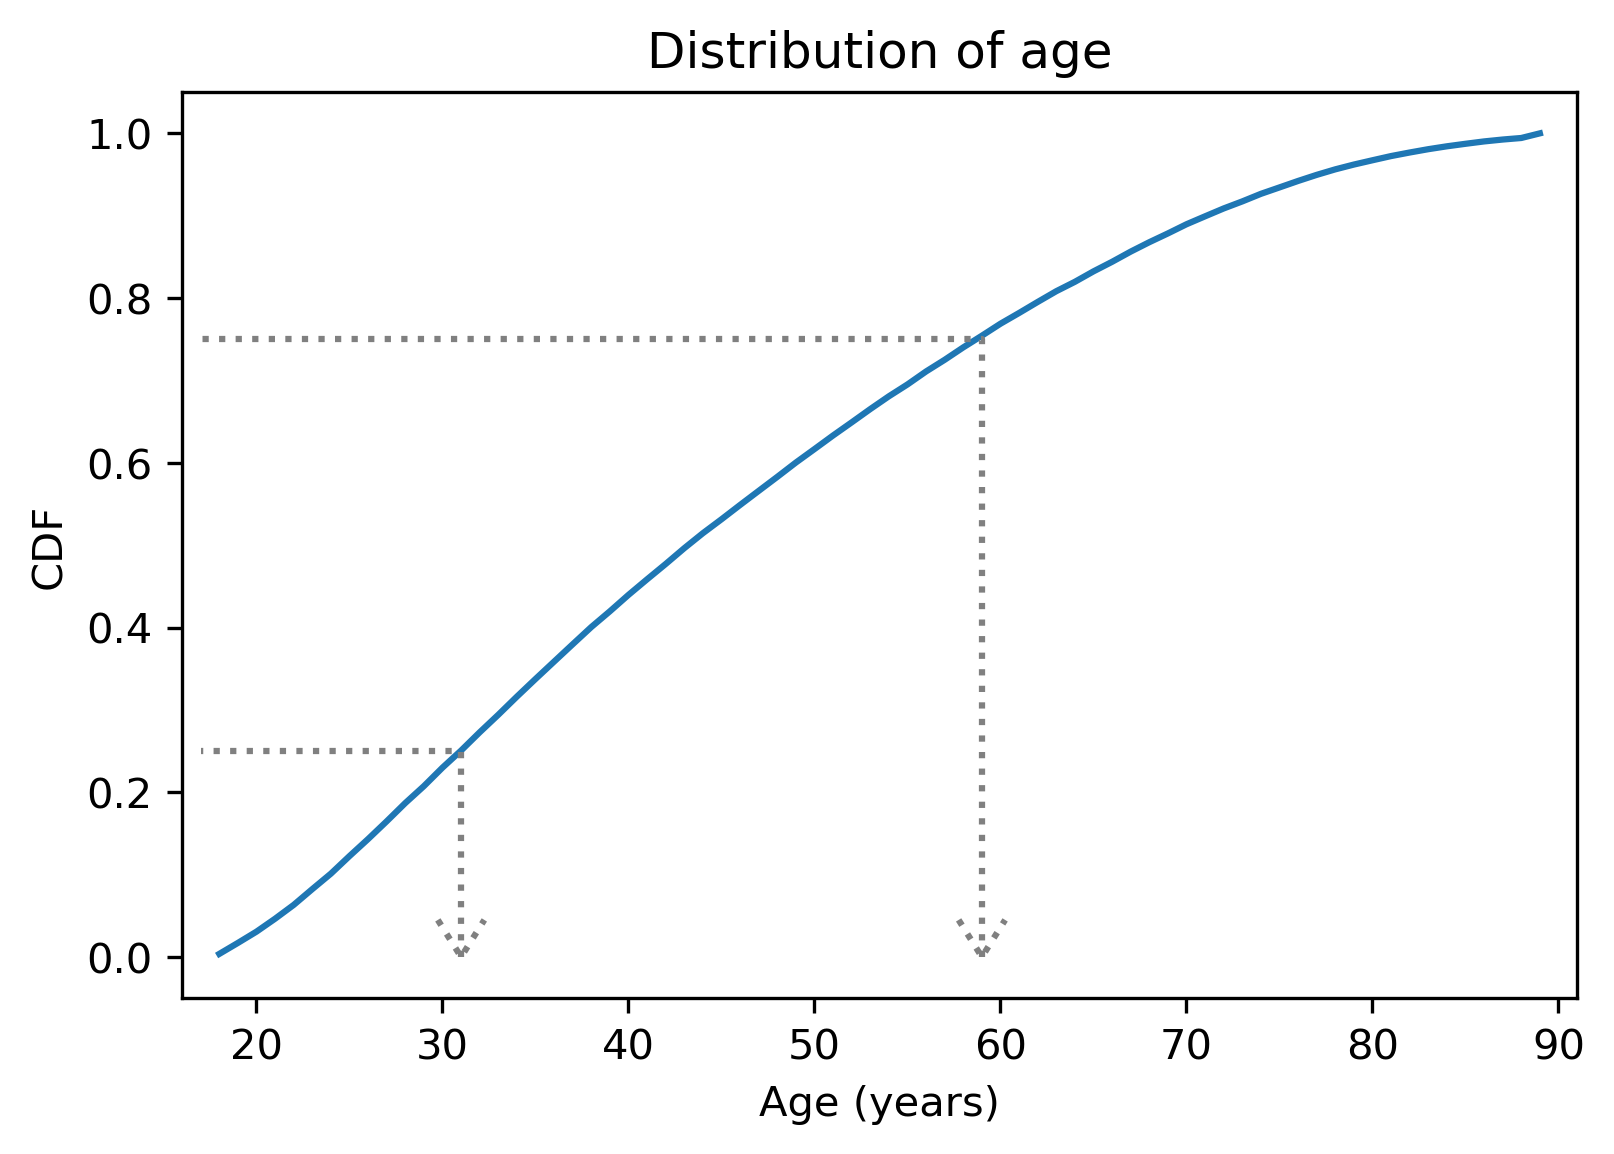
\includegraphics[scale=0.6666666]{08_distributions_files/08_distributions_78_0.png}
\end{center}

Because CDFs smooth out randomness, they provide a better view of real
differences between distributions. In this case, the lines are close
together until age 40 -- after that, the CDF is higher for men than
women.

So what does that mean? One way to interpret the difference is that the
fraction of men below a given age is generally more than the fraction of
women below the same age. For example, about 77\% of men are 60 or less,
compared to 75\% of women.

\begin{lstlisting}[language=Python,style=source]
cdf_male_age(60), cdf_female_age(60)
\end{lstlisting}

\begin{lstlisting}[style=output]
(array(0.7721998), array(0.7474241))
\end{lstlisting}

\pagebreak

Going the other way, we could also compare percentiles. For example, the
median age woman is older than the median age man, by about one year.

\begin{lstlisting}[language=Python,style=source]
cdf_male_age.inverse(0.5), cdf_female_age.inverse(0.5)
\end{lstlisting}

\begin{lstlisting}[style=output]
(array(44.), array(45.))
\end{lstlisting}

\textbf{Exercise:} What fraction of men are over 80? What fraction of
women?

\section{Comparing Incomes}\label{comparing-incomes}

As another example, let's look at household income and compare the
distribution before and after 1995 (I chose 1995 because it's roughly
the midpoint of the survey). We'll make two Boolean
\passthrough{\lstinline!Series!} objects to select respondents
interviewed before and after 1995.

\begin{lstlisting}[language=Python,style=source]
pre95 = (gss['year'] < 1995)
post95 = (gss['year'] >= 1995)
\end{lstlisting}

Now we can plot the PMFs of \passthrough{\lstinline!realinc!}, which
records household income converted to 1986 dollars.

\begin{lstlisting}[language=Python,style=source]
realinc = gss['realinc']

Pmf.from_seq(realinc[pre95]).plot(label='Before 1995')
Pmf.from_seq(realinc[post95]).plot(label='After 1995')

plt.xlabel('Income (1986 USD)')
plt.ylabel('PMF')
plt.title('Distribution of income')
plt.legend();
\end{lstlisting}

\begin{center}
\includegraphics[scale=0.6666666]{08_distributions_files/08_distributions_87_0.png}
\end{center}

There are a lot of unique values in this distribution, and none of them
appear very often. As a result, the PMF is so noisy and we can't really
see the shape of the distribution. It's also hard to compare the
distributions. It looks like there are more people with high incomes
after 1995, but it's hard to tell. We can get a clearer picture with a
CDF.

\begin{lstlisting}[language=Python,style=source]
Cdf.from_seq(realinc[pre95]).plot(label='Before 1995')
Cdf.from_seq(realinc[post95]).plot(label='After 1995')

plt.xlabel('Income (1986 USD)')
plt.ylabel('CDF')
plt.title('Distribution of income')
plt.legend();
\end{lstlisting}

\begin{center}
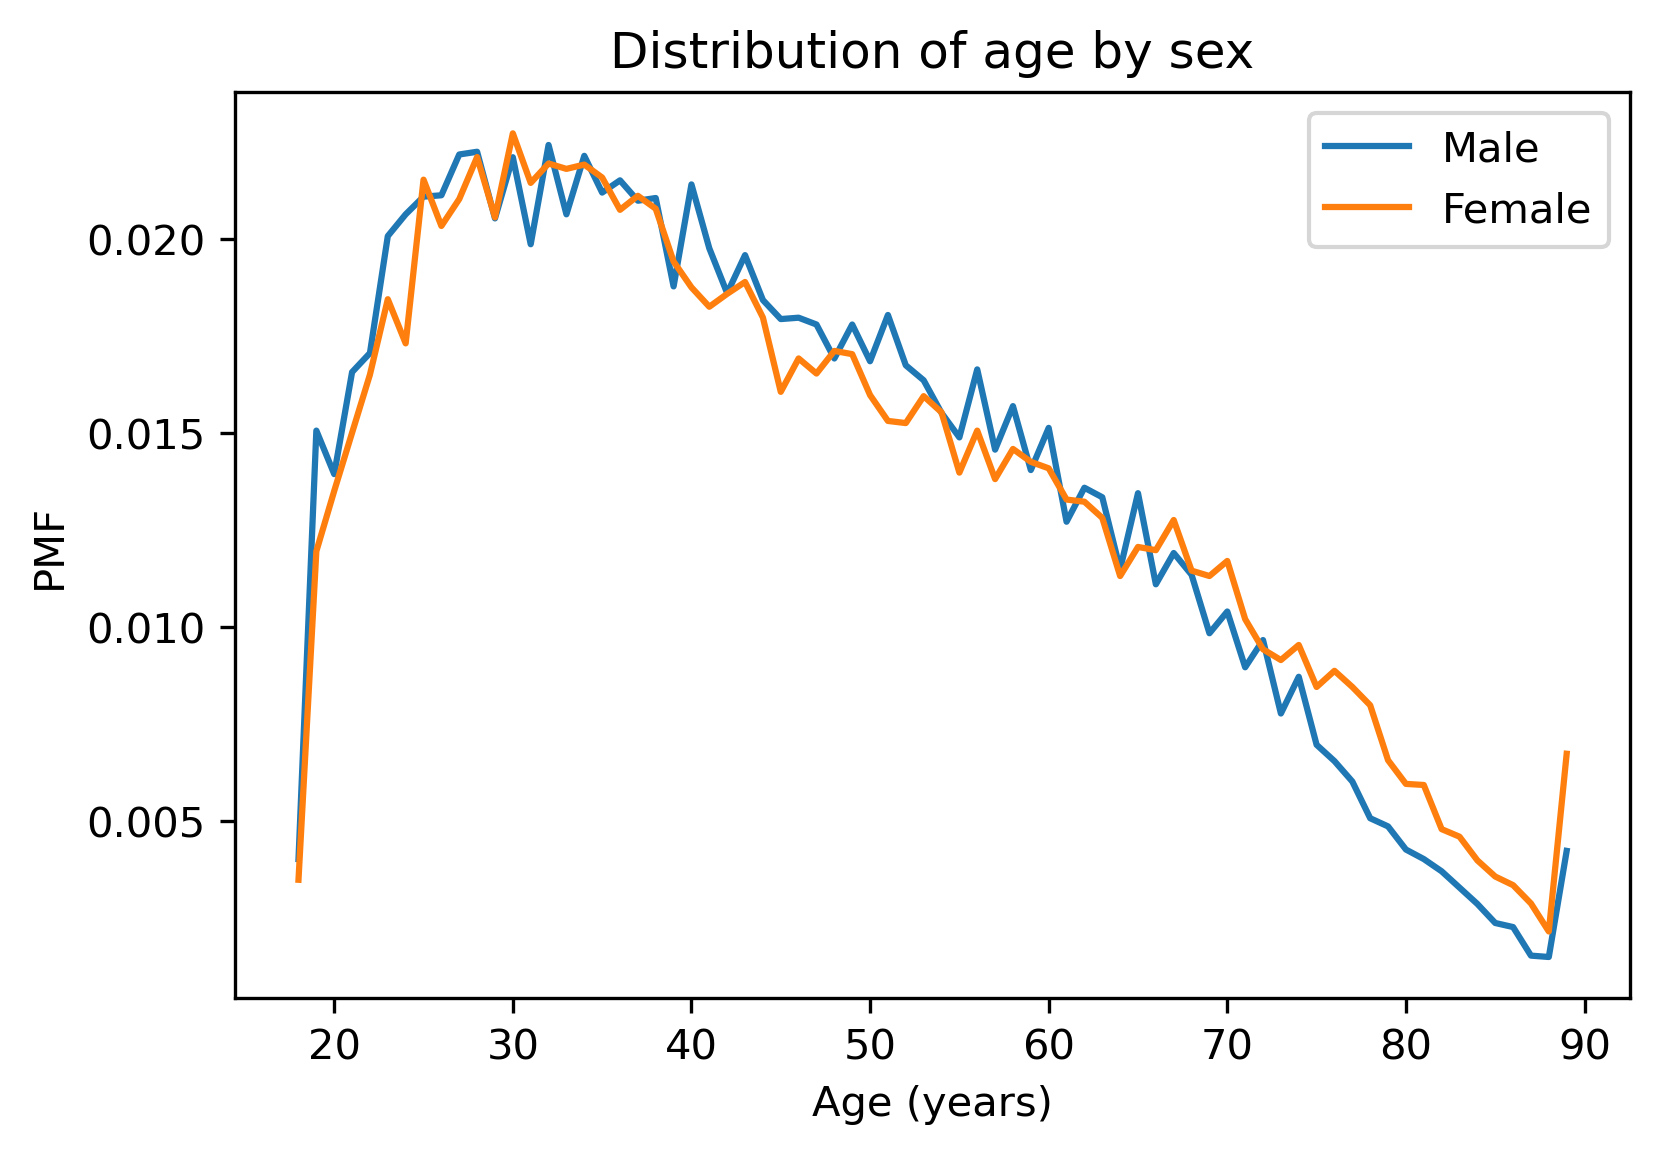
\includegraphics[scale=0.6666666]{08_distributions_files/08_distributions_89_0.png}
\end{center}

Below \$30,000 the CDFs are almost identical; above that, we can see
that the post-1995 distribution is shifted to the right. In other words,
the fraction of people with high incomes is about the same, but the
income of high earners has increased.

In general, I recommend CDFs for exploratory analysis. They give you a
clear view of the distribution, without too much noise, and they are
good for comparing distributions.

\textbf{Exercise:} Let's compare incomes for different levels of
education in the GSS dataset. We'll use the
\passthrough{\lstinline!degree!} column, which represents the highest
degree each respondent has earned. In this column, the value
\passthrough{\lstinline!1!} indicates a high school diploma,
\passthrough{\lstinline!2!} indicates an Associate's degree, and
\passthrough{\lstinline!3!} indicates a Bachelor's degree.

Compute and plot the distribution of income for each group. Remember to
label the CDFs, display a legend, and label the axes. Write a few
sentences that describe and interpret the results.

\section{Modeling Distributions}\label{modeling-distributions}

Some distributions have names. For example, you might be familiar with
the normal distribution, also called the Gaussian distribution or the
bell curve. And you might have heard of others like the exponential
distribution, binomial distribution, or maybe Poisson distribution.
These ``distributions with names'' are called \textbf{theoretical}
because they are based on mathematical functions, as contrasted with
empirical distributions, which are based on data.

Many things we measure have distributions that are well approximated by
theoretical distributions, so these distributions are sometimes good
models for the real world. In this context, what I mean by a
\textbf{model} is a simplified description of the world that is accurate
enough for its intended purpose.

To check whether a theoretical distribution is a good model for a
dataset, we can compare the CDF of the data to the CDF of a normal
distribution with the same mean and standard deviation. I'll demonstrate
with a sample from a normal distribution, then we'll try it with real
data.

The following statement uses NumPy's \passthrough{\lstinline!random!}
library to generate 1000 values from a normal distribution with mean 10
and standard deviation 1.

\begin{lstlisting}[language=Python,style=source]
sample = np.random.normal(10, 1, size=1000)
\end{lstlisting}

Here's what the empirical distribution of the sample looks like.

\begin{lstlisting}[language=Python,style=source]
cdf_sample = Cdf.from_seq(sample)
cdf_sample.plot(label='Random sample')

plt.xlabel('x')
plt.ylabel('CDF')
plt.legend();
\end{lstlisting}

\begin{center}
\includegraphics[scale=0.6666666]{08_distributions_files/08_distributions_97_0.png}
\end{center}

Now let's compute the CDF of a normal distribution with the actual
values of the mean and standard deviation.

\begin{lstlisting}[language=Python,style=source]
from scipy.stats import norm

qs = np.linspace(6, 14)
ps = norm(10, 1).cdf(qs)
\end{lstlisting}

First we import \passthrough{\lstinline!norm!} from
\passthrough{\lstinline!scipy.stats!}, which is a collection of
functions related to statistics. Then we use
\passthrough{\lstinline!linspace()!} to create an array of
equally-spaced values from -3 to 3 -- those are the
\passthrough{\lstinline!qs!} where we will evaluate the normal CDF.
Next, \passthrough{\lstinline!norm(10, 1)!} creates an object that
represents a normal distribution with mean 10 and standard deviation 1.
Finally, \passthrough{\lstinline!cdf!} computes the CDF of the normal
distribution, evaluated at each of the \passthrough{\lstinline!qs!}.

I'll plot the normal CDF with a gray line and then plot the CDF of the
data again.

\begin{lstlisting}[language=Python,style=source]
plt.plot(qs, ps, color='gray', label='Normal CDF')
cdf_sample.plot(label='Random sample')

plt.xlabel('x')
plt.ylabel('CDF')
plt.legend();
\end{lstlisting}

\begin{center}
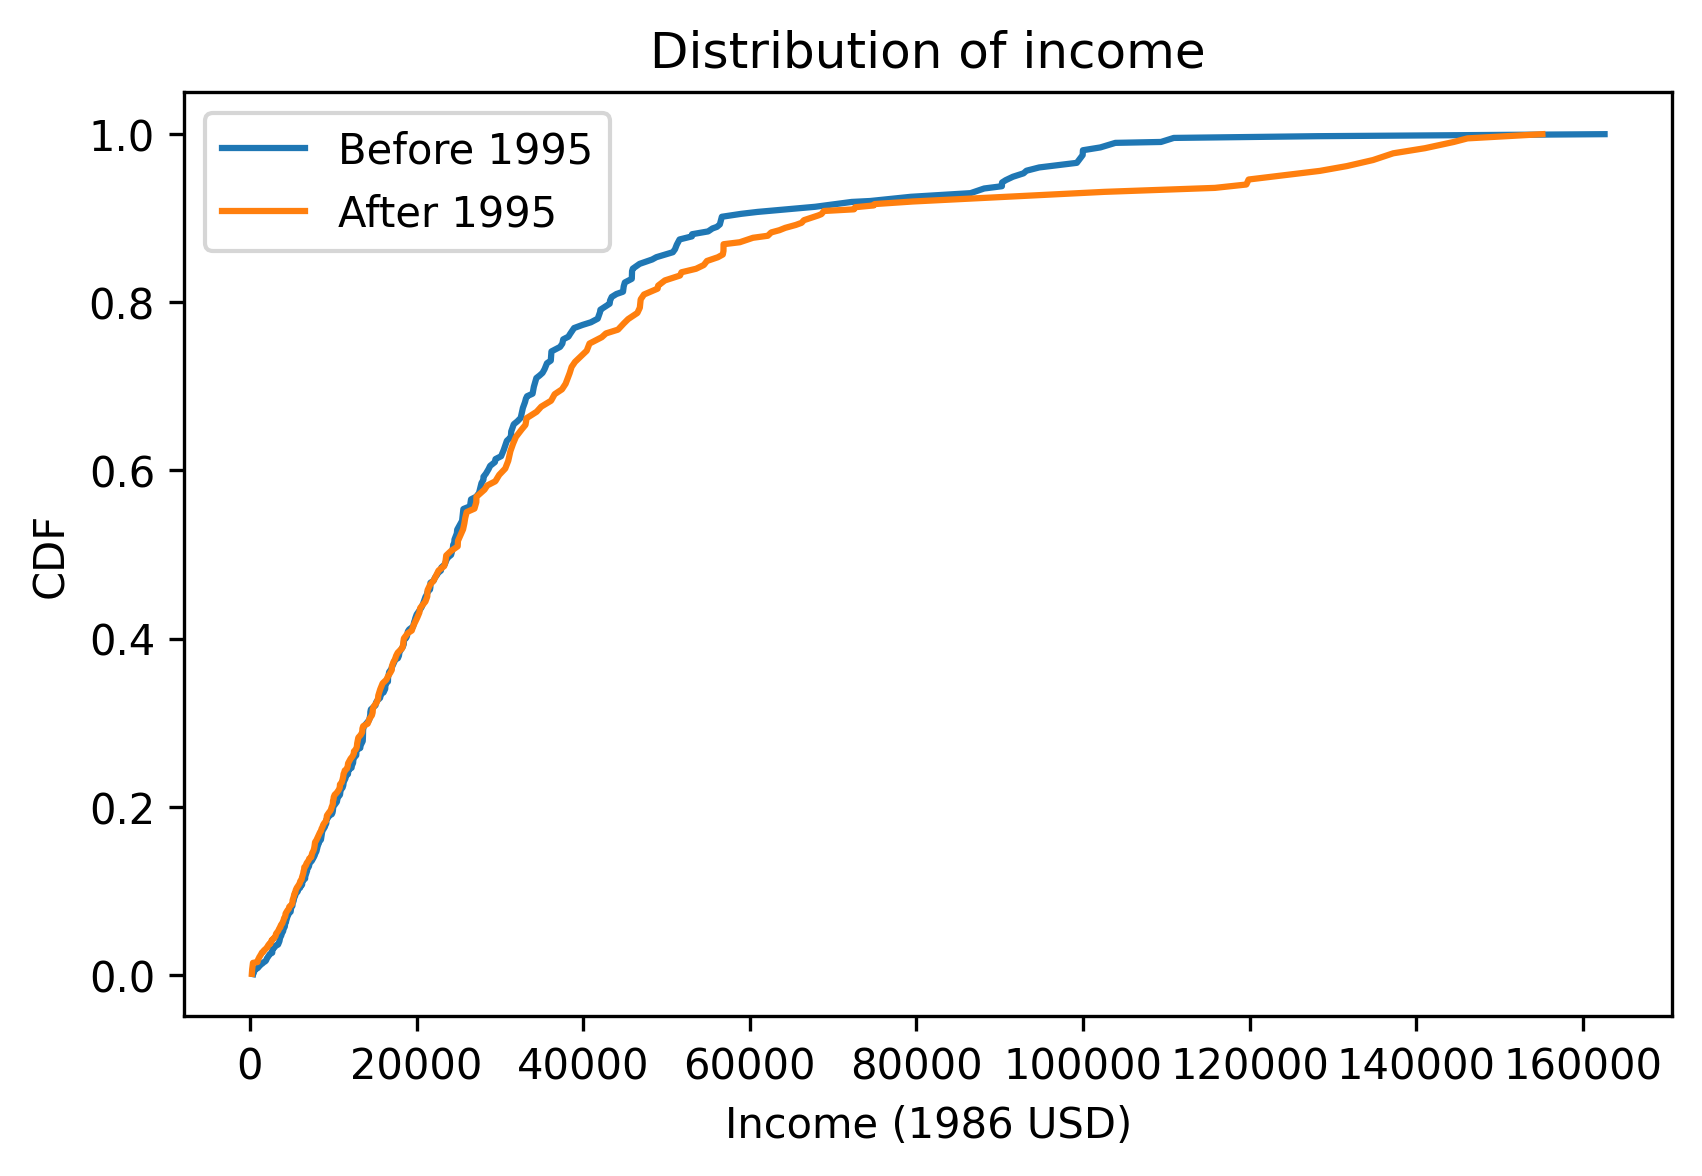
\includegraphics[scale=0.6666666]{08_distributions_files/08_distributions_101_0.png}
\end{center}

The CDF of the random sample agrees with the normal model -- which is
not surprising because the data were actually sampled from a normal
distribution. When we collect data in the real world, we do not expect
it to fit a normal distribution as well as this. In the next exercise,
we'll try it and see.

\textbf{Exercise:} In many datasets, the distribution of income is
approximately \textbf{lognormal}, which means that the logarithms of the
incomes fit a normal distribution. Let's see whether that's true for the
GSS data.

\begin{itemize}
\item
  Extract \passthrough{\lstinline!realinc!} from
  \passthrough{\lstinline!gss!} and compute the logarithms of the
  incomes using \passthrough{\lstinline!np.log10()!}.
\item
  Compute the mean and standard deviation of the log-transformed
  incomes.
\item
  Use \passthrough{\lstinline!norm!} to make a normal distribution with
  the same mean and standard deviation as the log-transformed incomes.
\item
  Plot the CDF of the normal distribution.
\item
  Compute and plot the CDF of the log-transformed incomes.
\end{itemize}

How similar are the CDFs of the log-transformed incomes and the normal
distribution?

\section{Kernel Density Estimation}\label{kernel-density-estimation}

We have seen two ways to represent distributions, PMFs and CDFs. Now
we'll learn another way: a probability density function, or PDF. The
\passthrough{\lstinline!norm!} function, which we used to compute the
normal CDF, can also compute the normal PDF.

\begin{lstlisting}[language=Python,style=source]
xs = np.linspace(6, 14)
ys = norm(10, 1).pdf(xs)
\end{lstlisting}

Here's what it looks like.

\begin{lstlisting}[language=Python,style=source]
plt.plot(xs, ys, color='gray', label='Normal PDF')

plt.xlabel('x')
plt.ylabel('PDF')
plt.title('Normal density function')
plt.legend();
\end{lstlisting}

\begin{center}
\includegraphics[scale=0.6666666]{08_distributions_files/08_distributions_108_0.png}
\end{center}

The normal PDF is the classic ``bell curve''. Now, it is tempting to
compare the PMF of the data to the PDF of the normal distribution, but
that doesn't work. Let's see what happens if we try:

\begin{lstlisting}[language=Python,style=source]
plt.plot(xs, ys, color='gray', label='Normal PDF')

pmf_sample = Pmf.from_seq(sample)
pmf_sample.plot(label='Random sample')

plt.xlabel('x')
plt.ylabel('PDF')
plt.title('Normal density function')
plt.legend();
\end{lstlisting}

\begin{center}
\includegraphics[scale=0.6666666]{08_distributions_files/08_distributions_110_0.png}
\end{center}

The PMF of the sample is a flat line across the bottom. In the random
sample, every value is unique, so they all have the same probability,
one in 1000.

However, we can use the points in the sample to estimate the PDF of the
distribution they came from. This process is called \textbf{kernel
density estimation}, or KDE. To generate a KDE plot, we'll use the
Seaborn library, imported as \passthrough{\lstinline!sns!}. Seaborn
provides \passthrough{\lstinline!kdeplot!}, which takes the sample,
estimates the PDF, and plots it.

\begin{lstlisting}[language=Python,style=source]
import seaborn as sns

sns.kdeplot(sample, label='Estimated sample PDF')

plt.xlabel('x')
plt.ylabel('PDF')
plt.title('Normal density function')
plt.legend();
\end{lstlisting}

\begin{center}
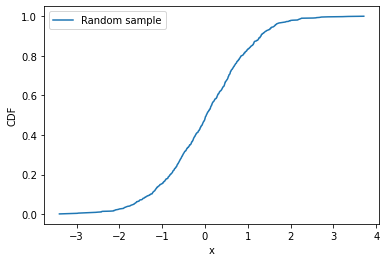
\includegraphics[scale=0.6666666]{08_distributions_files/08_distributions_112_0.png}
\end{center}

Now we can compare the KDE plot and the normal PDF.

\begin{lstlisting}[language=Python,style=source]
plt.plot(xs, ys, color='gray', label='Normal PDF')
sns.kdeplot(sample, label='Estimated sample PDF')

plt.xlabel('x')
plt.ylabel('PDF')
plt.title('Normal density function')
plt.legend();
\end{lstlisting}

\begin{center}
\includegraphics[scale=0.6666666]{08_distributions_files/08_distributions_114_0.png}
\end{center}

The KDE plot matches the normal PDF well. We can see places where the
data deviate from the model, but because we know the data really came
from a normal distribution, we know those deviations are due to random
sampling.

Comparing PDFs is a sensitive way to look for differences, but often it
is too sensitive -- it can be hard to tell whether apparent differences
mean anything, or if they are just random, as in this case.

\textbf{Exercise:} In a previous exercise, we used CDFs to see if the
distribution of income fits a lognormal distribution. We can make the
same comparison using a PDF and KDE.

\begin{itemize}
\item
  Again, extract \passthrough{\lstinline!realinc!} from
  \passthrough{\lstinline!gss!} and compute its logarithm using
  \passthrough{\lstinline!np.log10()!}.
\item
  Compute the mean and standard deviation of the log-transformed
  incomes.
\item
  Use \passthrough{\lstinline!norm!} to make a normal distribution with
  the same mean and standard deviation as the log-transformed incomes.
\item
  Plot the PDF of the normal distribution.
\item
  Use \passthrough{\lstinline!sns.kdeplot()!} to estimate and plot the
  density of the log-transformed incomes.
\end{itemize}

\section{Summary}\label{summary}

In this chapter, we've seen three ways to visualize distributions: PMFs,
CDFs, and KDE plots. In general, I use CDFs when I am exploring data --
that way, I get the best view of what's going on without getting
distracted by noise. Then, if I am presenting results to an audience
unfamiliar with CDFs, I might use a PMF if the dataset contains a small
number of unique values, or KDE if there are many unique values.
